\chapter{Comparación entre distintas implementaciones}

En este capítulo, se compara el rendimiento de diversas implementaciones de redes neuronales convolucionales (CNN). Primero, se presentan cinco modelos diferentes con configuraciones variadas en cuanto al tamaño de las imágenes de entrada, el número de capas convolucionales, de agrupación máxima, y neuronas en las capas totalmente conectadas, junto con diferencias en los hiperparámetros como el learning rate y el tamaño del mini-batch.

Luego, se utilizan dos bases de datos, CIFAR10 \cite{cifar10} y 10 Big Cats Of The Wild \cite{10_big_cats}, para entrenar y evaluar estos modelos. Los resultados muestran que el entrenamiento con el Modelo 1 en ambas bases de datos presenta una disminución en la entropía cruzada y un aumento en la precisión, confirmando la efectividad del modelo.

Finalmente, se realiza una comparación detallada de los tiempos de cómputo de las distintas implementaciones. En cuanto a las implementaciones en CPU, se observa una mejora significativa en el rendimiento al utilizar OpenMP en comparación con la implementación secuencial. En el caso de las implementaciones en GPU, aunque CUDA muestra una ligera mejora de rendimiento en modelos de menor complejidad, cuDNN ofrece un rendimiento superior en modelos más complejos. Por último, se presentan gráficos y una tabla que detallan los tiempos de ejecución de las operaciones en cada implementación.

\subsection{Modelos a emplear}

A continuación, se presenta la arquitectura general de algunos de los modelos que se utilizarán para medir el rendimiento y comparar las distintas implementaciones de redes neuronales convolucionales (CNN) desarrolladas a lo largo de este proyecto.

\begin{enumerate}
	\item \textbf{Modelo 0}
	\begin{enumerate}[label=\textbullet, nosep]
		\item Tamaño imágenes de entrada: 3x12x12
		\item Capas convolucionales
		\begin{enumerate}[label=\textbullet, nosep]
			\item 16 kernels de tamaño 3x3, padding=1
			\item 32 kernels de tamaño 3x3, padding=1
		\end{enumerate}
		\item Capas de Agrupación Máxima
		\begin{enumerate}[label=\textbullet, nosep]
			\item Kernel de tamaño 2x2
			\item Kernel de tamaño 2x2
		\end{enumerate}
		\item Capas totalmente conectadas
		\begin{enumerate}[label=\textbullet, nosep]
			\item n\_neuronas\_tras\_flatten
			\item 100 neuronas
			\item 10 neuronas
		\end{enumerate}
		\item learning rate = 0.01
		\item 1000 imágenes de entrenamiento
		\item Tamaño de mini batch = 32
	\end{enumerate}
	
	\item \textbf{Modelo 1}
	\begin{enumerate}[label=\textbullet, nosep]
		\item Tamaño imágenes de entrada: 3x32x32
		\item Capas convolucionales
			\begin{enumerate}[label=\textbullet, nosep]
				\item 16 kernels de tamaño 3x3, padding=1
				\item 32 kernels de tamaño 3x3, padding=1
			\end{enumerate}
		\item Capas de Agrupación Máxima
		\begin{enumerate}[label=\textbullet, nosep]
			\item Kernel de tamaño 2x2
			\item Kernel de tamaño 2x2
		\end{enumerate}
		\item Capas totalmente conectadas
		\begin{enumerate}[label=\textbullet, nosep]
			\item n\_neuronas\_tras\_flatten
			\item 100 neuronas
			\item 10 neuronas
		\end{enumerate}
		\item learning rate = 0.01
		\item 1000 imágenes de entrenamiento
		\item Tamaño de mini batch = 32
	\end{enumerate}
	
	\item \textbf{Modelo 2}
	\begin{enumerate}[label=\textbullet, nosep]
		\item Tamaño imágenes de entrada: 3x40x40
		\item Capas convolucionales
		\begin{enumerate}[label=\textbullet, nosep]
			\item 16 kernels de tamaño 3x3, padding=1
			\item 32 kernels de tamaño 3x3, padding=1
		\end{enumerate}
		\item Capas de Agrupación Máxima
		\begin{enumerate}[label=\textbullet, nosep]
			\item Kernel de tamaño 2x2
			\item Kernel de tamaño 2x2
		\end{enumerate}
		\item Capas totalmente conectadas
		\begin{enumerate}[label=\textbullet, nosep]
			\item n\_neuronas\_tras\_flatten
			\item 100 neuronas
			\item 10 neuronas
		\end{enumerate}
		\item learning rate = 0.001
		\item 1000 imágenes de entrenamiento
		\item Tamaño de mini batch = 32
	\end{enumerate}
	
	\item \textbf{Modelo 3}
	\begin{enumerate}[label=\textbullet, nosep]
		\item Tamaño imágenes de entrada: 3x40x40
		\item Capas convolucionales
		\begin{enumerate}[label=\textbullet, nosep]
			\item 16 kernels de tamaño 3x3, padding=1
			\item 32 kernels de tamaño 3x3, padding=1
			\item 32 kernels de tamaño 3x3, padding=1
		\end{enumerate}
		\item Capas de Agrupación Máxima
		\begin{enumerate}[label=\textbullet, nosep]
			\item Kernel de tamaño 2x2
			\item Kernel de tamaño 2x2
			\item Kernel de tamaño 2x2
		\end{enumerate}
		\item Capas totalmente conectadas
		\begin{enumerate}[label=\textbullet, nosep]
			\item n\_neuronas\_tras\_flatten
			\item 128 neuronas
			\item 50 neuronas
			\item 10 neuronas
		\end{enumerate}
		\item learning rate = 0.00001
		\item 2000 imágenes de entrenamiento
		\item Tamaño de mini batch = 32
	\end{enumerate}	
	
	\item \textbf{Modelo 4}
	\begin{enumerate}[label=\textbullet, nosep]
		\item Tamaño imágenes de entrada: 3x50x50
		\item Capas convolucionales
		\begin{enumerate}[label=\textbullet, nosep]
			\item 32 kernels de tamaño 3x3, padding=1
			\item 32 kernels de tamaño 3x3, padding=1
			\item 32 kernels de tamaño 3x3, padding=1
		\end{enumerate}
		\item Capas de Agrupación Máxima
		\begin{enumerate}[label=\textbullet, nosep]
			\item Kernel de tamaño 2x2
			\item Kernel de tamaño 2x2
			\item Kernel de tamaño 2x2
		\end{enumerate}
		\item Capas totalmente conectadas
		\begin{enumerate}[label=\textbullet, nosep]
			\item n\_neuronas\_tras\_flatten
			\item 200 neuronas
			\item 50 neuronas
			\item 10 neuronas
		\end{enumerate}
		\item learning rate = 0.00001
		\item 2500 imágenes de entrenamiento
		\item Tamaño de mini batch = 32
	\end{enumerate}		

	
\end{enumerate}

\subsection{Bases de datos}

Se utilizará una variedad de bases de datos en el presente estudio. Entre ellas, se incluyen los resultados obtenidos durante el entrenamiento con las bases de datos CIFAR10 \cite{cifar10}, y 10 Big Cats Of The Wild \cite{10_big_cats}, ambas caracterizadas por ser problemas de clasificación multiclase con 10 clases distintas. En CIFAR10, las 10 clases representan aviones, automóviles, pájaros, gatos, ciervos, perros, ranas, caballos, barcos y camiones. Por otro lado, en 10 Big Cats, las 10 clases representan el leopardo africano, caracal, guepardo, leopardo nublado, jaguar, leones, ocelote, puma, leopardo de las nieves y tigre. Además, para cada clase se utilizará el mismo número de imágenes.

\subsection{Resultados en entrenamiento}

En esta sección, se utiliza el \texttt{Modelo 1} previamente definido, para su entrenamiento en diversos conjuntos de datos, y se analizan los resultados obtenidos. La evaluación de los resultados se realiza mediante el uso de la entropía cruzada como función de error, y la precisión como métrica de efectividad. En relación con los resultados de las distintas implementaciones, todas ellas producen los mismos resultados. Esto es consistente con el hecho de que cada implementación se basa en la anterior y le incorpora algún tipo de mejora. Asimismo, se han llevado a cabo diversas pruebas, como fijar los valores iniciales de los pesos, así como los datos de entrada, y la estructura de una red neuronal convolucional (CNN) específica. Con estos tres aspectos establecidos, se ha procedido a realizar la propagación hacia delante de los mismos datos a lo largo de cada CNN (una por cada implementación), observando que todas las implementaciones producen resultados idénticos, tanto en cada capa como en la predicción final. Además, los gradientes calculados para cada parámetro de la red en cada capa también coinciden. En consecuencia, se puede concluir que todas las implementaciones producen resultados equivalentes en términos de entropía cruzada y precisión. 

\begin{figure}[H]
	\centering
	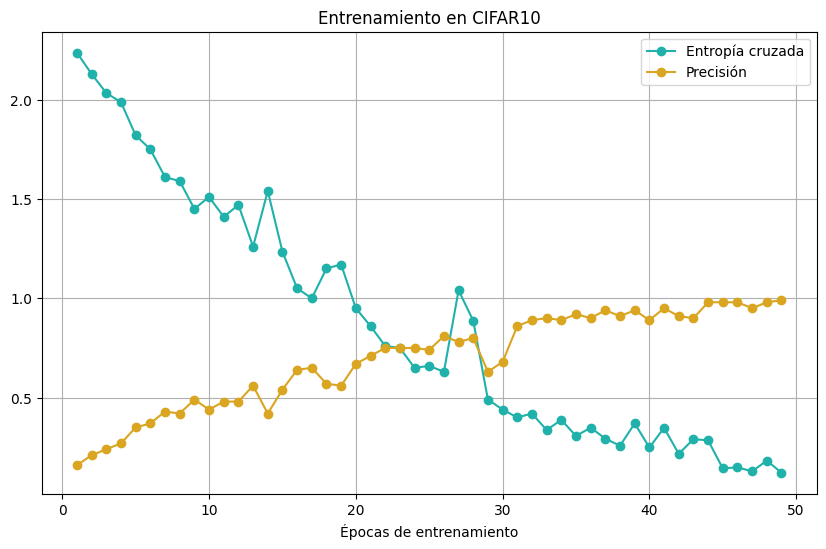
\includegraphics[scale=0.5]{imagenes/cifar10.png}  
	\caption{Entrenamiento con CIFAR10}
	\label{fig:cifar10}
\end{figure}

En la Figura \ref{fig:cifar10}, se presentan los resultados obtenidos durante el entrenamiento del \texttt{Modelo 1}, utilizando los datos del conjunto \texttt{CIFAR10} \cite{cifar10}. En dicha figura, el eje X representa las épocas de entrenamiento, mientras que el eje Y muestra la entropía cruzada o la precisión alcanzada en cada época, correspondientes a las gráficas azul y naranja, respectivamente. Se observa que, a medida que avanza el entrenamiento, la entropía cruzada disminuye progresivamente, mientras que la precisión aumenta. Este comportamiento es coherente con lo discutido en secciones anteriores, y refleja cómo el modelo mejora su capacidad para aprender las relaciones presentes en los datos de entrenamiento, incrementando gradualmente su precisión en las predicciones. 

\begin{figure}[H]
	\centering
	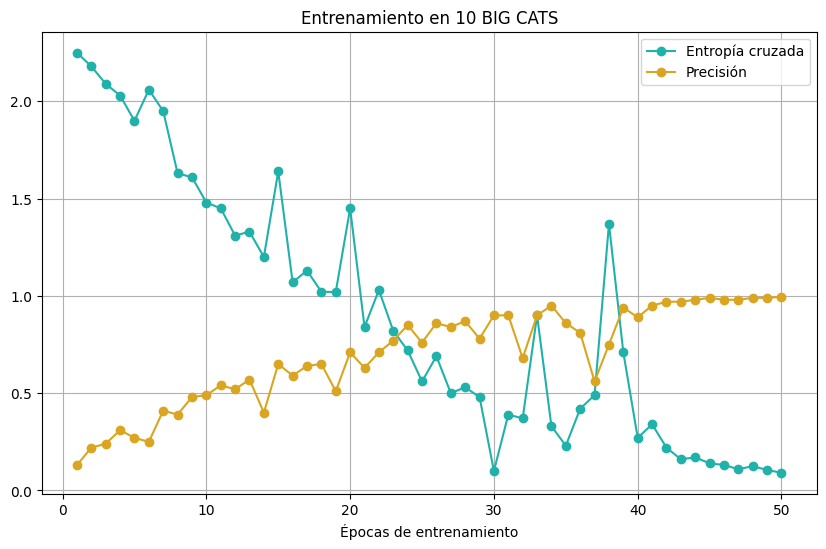
\includegraphics[scale=0.5]{imagenes/10_big_cats.png}  
	\caption{Entrenamiento con 10 Big Cats}
	\label{fig:10_big_cats}
\end{figure}

De manera similar, la Figura \ref{fig:10_big_cats} ilustra los resultados obtenidos durante el proceso de entrenamiento del \texttt{Modelo 1}, utilizando los datos del conjunto \texttt{10 Big Cats Of The Wild} \cite{10_big_cats}. En esta figura, se puede observar el rendimiento del modelo a lo largo de las diferentes épocas de entrenamiento, destacándose la evolución tanto de la entropía cruzada como de la precisión a lo largo del tiempo. El comportamiento observado en esta figura proporciona información valiosa sobre la capacidad del modelo para aprender patrones y relaciones específicas dentro de este conjunto de datos, lo cual es fundamental para evaluar su efectividad en tareas de clasificación relacionadas con la base de datos \texttt{10 Big Cats}.

\subsection{Comparación de rendimiento}

En esta sección, se compararán las prestaciones de cada implementación. Dado que todas producen los mismos resultados (una vez eliminados factores aleatorios como inicialización de pesos, entre otros), la comparación se centrará en el tiempo de cómputo requerido por cada una. \\
Se inicia el análisis con las implementaciones que requieren mayor tiempo de cómputo. Es decir, aquellas que emplean exclusivamente CPU, (Secuencial y OpenMP). Posteriormente, el análisis se enfocará en el rendimiento de los sistemas heterogéneos que emplean tanto CPU como GPU (CUDA y cuDNN). \\
Además, se presentan figuras que facilitan la comprensión  de los análisis de rendimiento, junto con una tabla que detalla los tiempos exactos empleados por cada capa de una misma arquitectura, desarrollada en distintas implementaciones.

\subsubsection{Implementaciones CPU}

\begin{figure}[H]
	\centering
	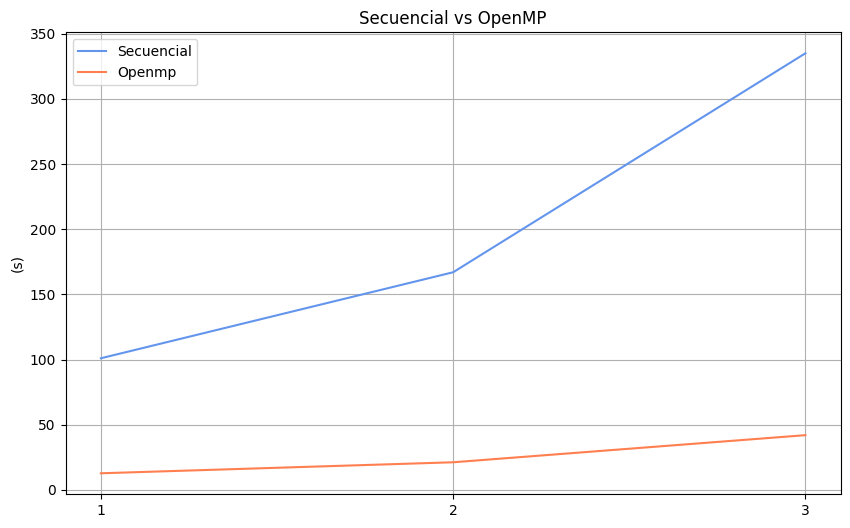
\includegraphics[scale=0.5]{imagenes/sec_openmp.png}  
	\caption{Secuencial vs OpenMP}
	\label{fig:sec_openmp}
\end{figure}

En la Figura \ref{fig:sec_openmp} se presenta una comparación de rendimiento entre la implementación secuencial y la implementación en OpenMP. El eje Y muestra el tiempo requerido en el entrenamiento de una época, mientras que el eje X indica el modelo empleado para dicho entrenamiento. De esta manera, el punto p1(100, 0) señala que el modelo 0 requiere 101 segundos para entrenar una época con la implementación secuencial, mientras que solo necesita 12.76 segundos con la implementación en OpenMP.

\begin{figure}[H]
	\centering
	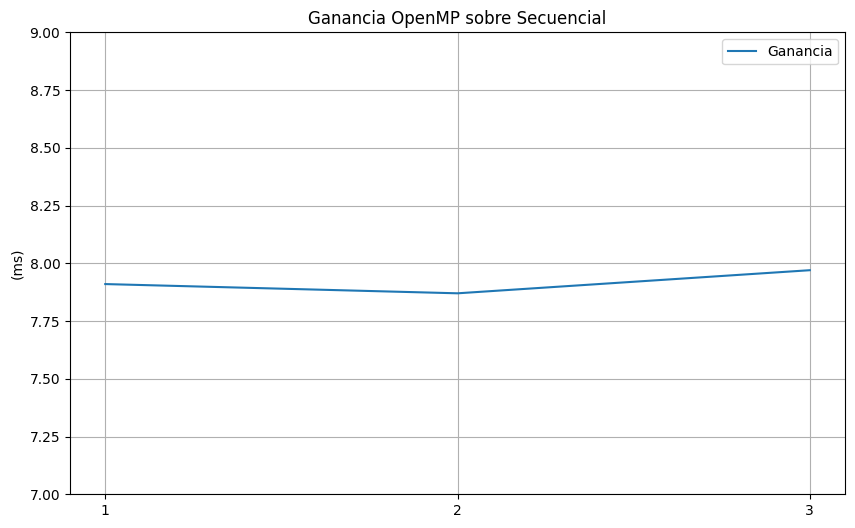
\includegraphics[scale=0.5]{imagenes/ganancia_sec_openmp.png}  
	\caption{Ganancia de OpenMP respecto a secuencial}
	\label{fig:ganancia_sec_openmp}
\end{figure}

La implementación utilizando OpenMP está diseñada para explotar el paralelismo a nivel de CPU mediante el uso de 8 hilos. Por lo tanto, se anticipa una mejora de rendimiento cercana a un factor de 8 en comparación con la implementación secuencial, como se muestra en la Figura \ref{fig:ganancia_sec_openmp}.

\vspace{10mm}

\subsubsection{Implementaciones GPU}

\begin{figure}[H]
	\centering
	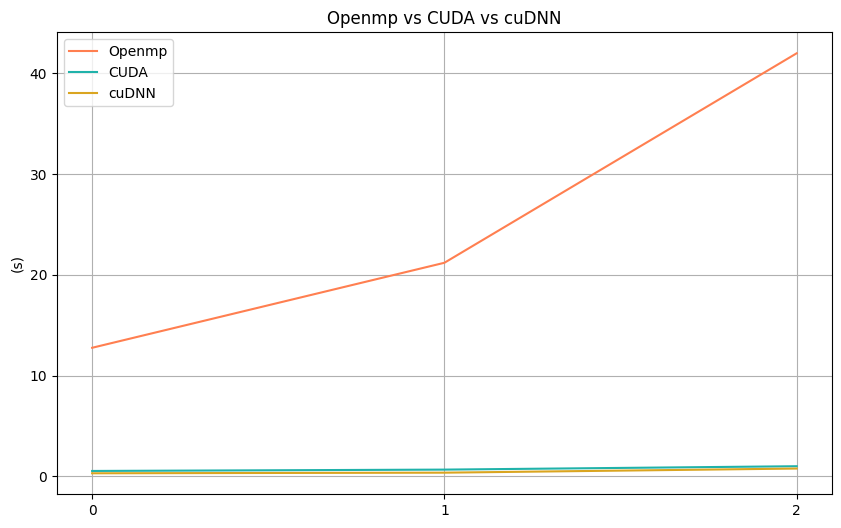
\includegraphics[scale=0.52]{imagenes/openmp_cuda_cudnn.png}  
	\caption{OpenMP vs CUDA vs CUDNN}
	\label{fig:openmp_cuda_cudnn}
\end{figure}

En la Figura \ref{fig:openmp_cuda_cudnn}, se utiliza los mismos modelos que se emplearon en las Figuras \ref{fig:sec_openmp} y \ref{fig:ganancia_sec_openmp}.
De manera similar a cómo la implementación en OpenMP presenta una mejora notable respecto a la implementación secuencial, también se espera una diferencia significativa entre las implementaciones heterogéneas que combinan CPU y GPU  y aquellas que se basan exclusivamente en el uso de CPU, como es el caso de OpenMP. Esta diferencia de rendimiento es particularmente evidente en las Figuras \ref{fig:openmp_cuda_cudnn} y \ref{fig:ganancia_cuda_cudnn_openmp}, donde las variaciones observadas en el rendimiento son incluso más pronunciadas que las reportadas en el apartado anterior.

\begin{figure}[H]
	\centering
	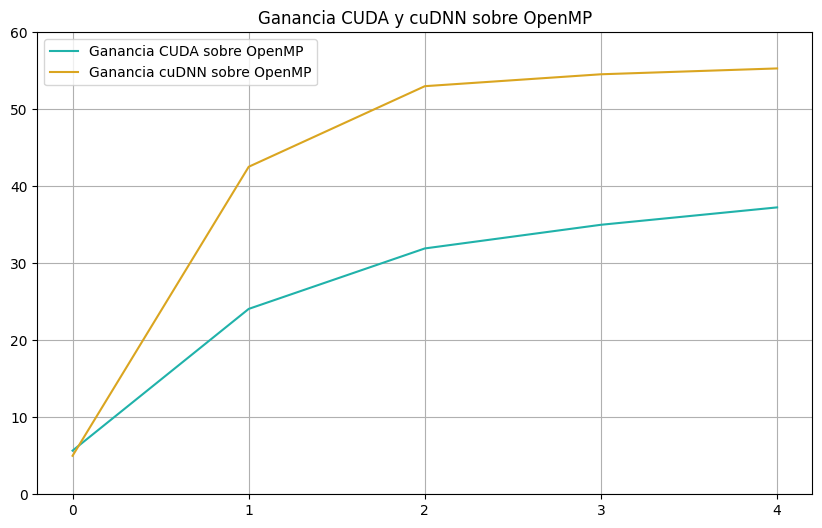
\includegraphics[scale=0.5]{imagenes/ganancia_cuda_cudnn_openmp.png}  
	\caption{Ganancia de CUDA y cuDNN sobre OpenMP}
	\label{fig:ganancia_cuda_cudnn_openmp}
\end{figure}

Para comparar las implementaciones en GPU, se han añadido dos modelos adicionales: uno de menor complejidad, \texttt{Modelo 0}, y otro de mayor complejidad, \texttt{Modelo 4}, en relación con los modelos previamente evaluados. Al igual que en el experimento anterior, estos modelos están dispuestos en las figuras de izquierda a derecha, organizados de menor a mayor complejidad. Este orden tiene como objetivo facilitar la comparación entre las distintas implementaciones en función de la complejidad creciente de los modelos.

\begin{figure}[H]
	\centering
	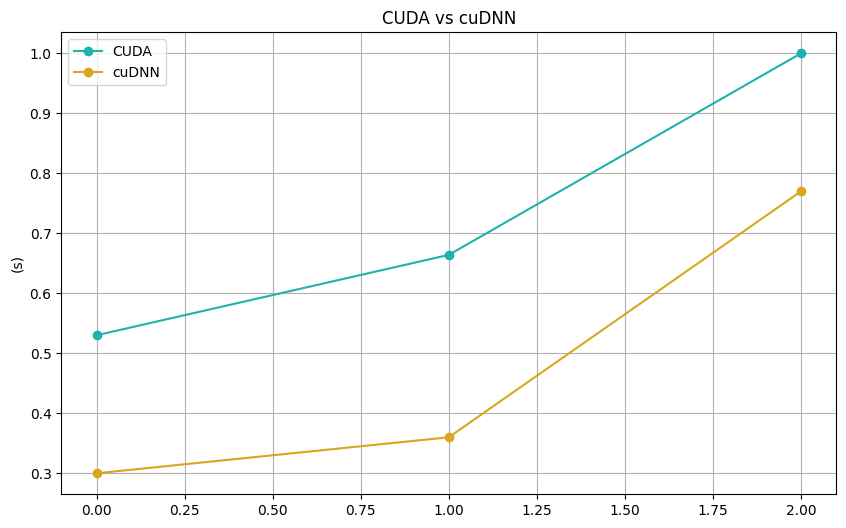
\includegraphics[scale=0.52]{imagenes/cuda_cudnn_1.png}  
	\caption{CUDA vs CUDNN}
	\label{fig:cuda_cudnn_1}
\end{figure}

Como se ilustra en la Figura \ref{fig:cuda_cudnn_1}, la implementación CUDA muestra un rendimiento ligeramente superior en modelos menos complejos. Sin embargo, a medida que aumenta la complejidad de los modelos, la implementación cuDNN comienza a superar a CUDA. Esta característica distintiva ha llevado a que cuDNN sea utilizada en numerosas librerías de alto nivel y prestigio, como Caffe2, MATLAB, PyTorch y TensorFlow, entre otras. 

\begin{table}[H]
	\centering
	\begin{tabular}{llll}
		Operación 	 &\vline  & CuDNN (ms) & CUDA (ms)  \\
		\hline
		
		Conv\_fwd\_0    & \vline & 0.005	 &	0.009 \\			
		Conv\_back\_0   & \vline & 	0.032 &	0.044 \\
		\hline
		Pool\_fwd\_0 	 & \vline & 0.003	 &	0.005 \\
		Pool\_back\_0 	 & \vline & 0.01    &	0.023 \\
		\hline
		\hline
		\hline
		Conv\_fwd\_1    & \vline & 0.02	 &	0.022	\\			
		Conv\_back\_1   & \vline & 0.065	 &	0.16	\\
		\hline
		Pool\_fwd\_1 	 & \vline & 0.0029	 &	0.0039	 \\
		Pool\_back\_1 	 & \vline  & 0.014    &	0.025	 \\
		\hline
		\hline
		\hline
		Conv\_fwd\_2    & \vline & 0.023	 &	0.018 \\			
		Conv\_back\_2   & \vline & 0.047	 &	0.018 \\
		\hline
		Pool\_fwd\_2 	 & \vline & 0.032	 &	0.023 \\
		Pool\_back\_2 	 & \vline & 0.0057    &	0.023 \\	
	\end{tabular}
	\caption{Comparación rendimiento CuDNN vs CUDA}
	\label{tabla_resultados}
\end{table}

Utilizando el modelo con la mayor complejidad mostrado en la Figura \ref{fig:cuda_cudnn_1}, \texttt{Modelo 4}, se ha generado la Tabla \ref{tabla_resultados}, la cual detalla el tiempo requerido para llevar a cabo tanto la propagación hacia delante como la retroprogación en cada capa del modelo. En dicha tabla, la notación Conv\_fwd\_i representa el tiempo de propagación hacia adelante en la capa convolucional i, Conv\_back\_i denota el tiempo de retropropagación en la capa convolcional i, Pool\_fwd\_i indica el tiempo de propagación hacia delante en la capa de agrupación máxima i, y Pool\_back\_0 indica el tiempo de retropropagación en la capa de agrupación máxima i.
Se observa en la tabla que, a medida que los datos avanzan a través de las distintas capas de la red neuronal convolucional (CNN), la ventaja inicial que cuDNN tenía sobre CUDA tiende a disminuir. Este comportamiento es coherente con la observación anterior, ya que en cada capa el coste computacional tiende a reducirse, (aunque no siempre es el caso, en el contexto específico de este modelo sí se cumple).